% v16 framework draft (2026-11-08): the paper reframed as an analysis of the positional
% cost of topology. Storyline and figure plan: notes/2026-11-08-framework-reframe.md.
% Build: tectonic -X compile framework_v16_en.tex
% Figures marked [TO DO] are stand-ins or placeholders; see the figure plan.
\documentclass[review]{vgtc}
\usepackage[T1]{fontenc}
\usepackage{mathptmx}
\usepackage{cite}
\usepackage{amsmath,amssymb,amsthm}
\usepackage{placeins}
\usepackage{booktabs,multirow,colortbl}

\makeatletter
\setlength{\@dblfptop}{0pt}
\setlength{\@dblfpsep}{12pt}
\setlength{\@dblfpbot}{0pt plus 1fil}
\makeatother
\setcounter{secnumdepth}{3}
\newtheorem{theorem}{Theorem}
\newtheorem{proposition}{Proposition}
\newcommand{\dtop}{d_{\mathrm{top}}}
\newcommand{\lca}{\operatorname{lca}}
\newcommand{\nroe}{\mathrm{NROE}}
\newcommand{\todo}[1]{{\color{red}\textbf{[TO DO: #1]}}}
\newcommand{\figplaceholder}[2]{\fbox{\parbox{#1}{\centering\small\color{red}\textbf{[Figure to be produced]}\\[2pt]\raggedright #2}}}
\title{The Positional Cost of Topology\\in Temporal Merge Tree Maps}
\author{Anonymous Authors}
\onlineid{1037}
\vgtccategory{Research}
\vgtcinsertpkg
\hypersetup{pdftitle={The Positional Cost of Topology in Temporal Merge Tree Maps},pdfauthor={Anonymous Authors}}
\abstract{A static overview of a time-varying scalar field gives space a single axis. Temporal merge tree maps keep the merge tree on this axis and place features for other goals, such as temporal coherence or relative distances. Any such layout distorts spatial relationships, but how much of the distortion is unavoidable, and where it arises, has remained open. We answer this question for position along a fixed spatial direction. We place merge tree maps and other one-dimensional linearizations in one position--topology plane and derive lower bounds on the displacement that every map must accept when it keeps the merge tree exactly, when features have finite widths, and when merge levels may change by a bounded amount. The bounds depend only on the tree, the projected feature locations and the widths. They name the merges that force the displacement and the merge error that releases it, and they split the positional error of any map into a part forced by the hierarchy and a part chosen by its layout. On seven planar and volumetric sequences, 31--95\% of the order error of three topology-preserving orderings, including TMTM and ST-MTM, is not forced by the tree; the forced part changes by up to a factor of five with the direction; and a construction that follows the bounds attains them on 606 of 614 planar frames. On the four planar inputs of the ST-MTM benchmark, such anchored maps place features 73--96\% closer to their projected locations, while ST-MTM preserves neighborhoods better.}
\keywords{Time-varying scalar fields, merge tree maps, topology preservation, spatial fidelity, lower bounds, constrained layout.}
\teaser{
\centering
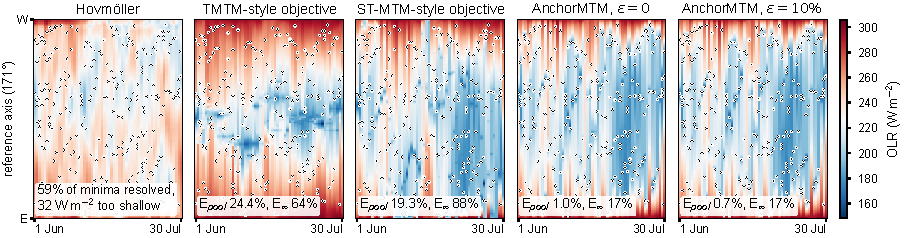
\includegraphics[width=\linewidth]{../figures/fw_olr_maps.pdf}
\par
\refstepcounter{figure}\label{fig:teaser}
{\captionfonts\raggedright\noindent\figurename~\thefigure: Existing merge tree maps place features far from their locations, and most of that distance is not forced by the merge tree. Sixty days of outgoing longwave radiation along one spatial direction (west at the top). Black dots: projected locations of the minima. Left: the Hovm\"oller diagram keeps the coordinate but averages nearby minima into one dip. Middle: objectives modelled on TMTM and ST-MTM keep every merge tree but leave features 24.4\% and 19.3\% of the axis from their locations on average. Right: maps that follow the bounds of Section~\ref{sec:bounds} keep the trees and their features within 1.0\% on average. \todo{add under each merge tree map a bar splitting its order error into the part forced by the tree ($\nu^*$, 0.89\%) and the part chosen by its layout}\par}
}
\linespread{0.90}
\setlength{\textfloatsep}{7pt}
\setlength{\floatsep}{6pt}
\setlength{\dbltextfloatsep}{7pt}
\begin{document}
\firstsection{Introduction}
\maketitle
\raggedbottom
\setlength{\emergencystretch}{1.5em}
Analysts who study storms, convection or wildfires compare features across hundreds of time steps. Animation keeps the spatial view of each instant but makes distant times hard to compare; a static overview shows all times at once by giving time one axis and compressing space into the other~\cite{Tversky:2002:Animation,Robertson:2008:Animation,Bach:2017:STC}. What the spatial axis means decides what the overview can show.

Temporal merge tree maps make the merge tree the organizing principle of that axis. TMTM linearizes each frame by a traversal of its augmented merge tree, so the one-dimensional profile has the same merge tree as the field, and aligns the traversals over time~\cite{Koepp:2023:TMTM}. ST-MTM keeps the hierarchy and fits the distances between features~\cite{STMTM:2026}. Both keep the tree exactly; position on their axis serves temporal coherence or relative distances. The ST-MTM authors observe that no one-dimensional layout can preserve all spatial relationships, so a nonzero distortion is expected of every method rather than a sign of its failure~\cite{STMTM:2026}. This leaves open how much distortion is expected, that is, forced by the data and the hierarchy, and how much is chosen by a method.

We answer this question for the most direct spatial reading of the axis: position along one fixed spatial direction, the coordinate that a Hovm\"oller diagram keeps~\cite{Hovmoller:1949}. Project every extremum onto the direction; a map is faithful to this reading to the extent that it places each feature near its projection. The merge tree prevents this in general. The features of one subtree must occupy one block of the axis, yet their projections can interleave with those of another subtree (Fig.~\ref{fig:concept}), so some displacement is forced. We ask how much, where it arises, and what it would take to remove it.

We place merge tree maps and other linearizations in one \emph{position--topology plane}: each map is a point given by the merge error of its displayed profile and the displacement of its features from their projections. On this plane we derive lower bounds that no map can cross, for exact topology, for finite feature widths and for a bounded merge error. They depend only on the tree, the projections and the widths, need no layout and take milliseconds per frame. Each bound names the sibling subtrees whose projected ranges overlap and the merge error at which they may interleave, and it splits the positional error of any map into a part forced by the hierarchy and a part chosen by its layout.

Measured against these bounds, the forced cost on real planar data is small, 0.9--5.8\% of the axis in order error, while topology-preserving orderings such as TMTM and ST-MTM exceed it severalfold: 31--95\% of their order error is not forced by the tree. The forced cost depends on where the conflicting subtrees merge and on the chosen direction, which can change it by a factor of five. A construction that follows the bounds attains them on 606 of 614 real planar frames, so the bounds are tight, and its maps carry a known positional error (Fig.~\ref{fig:teaser}).

Our contributions are:
\begin{itemize}
\setlength{\itemsep}{2pt}
\setlength{\parsep}{0pt}
\item a common model that places merge tree maps and other one-dimensional linearizations in one position--topology plane, measured by the merge error of the displayed profile and the displacement of features from a fixed spatial reference (Section~\ref{sec:model});
\item lower bounds on this plane for exact topology, finite widths and a bounded merge error, which name the merges that force the displacement and the merge error that releases it, and which split the error of any map into forced and chosen parts (Section~\ref{sec:bounds});
\item a characterization on seven sequences and the ST-MTM benchmark of how large the forced cost is, where it arises, how far existing maps exceed it and how it depends on the direction, together with a construction that attains the bounds (Sections~\ref{sec:attain} and~\ref{sec:experiments}).
\end{itemize}

\section{Related Work}\label{sec:related}
\paragraph{Merge tree maps and topological landscapes.} Topological landscapes and their profiles turn a merge or contour tree into a terrain or a one-dimensional function with the same topology~\cite{Weber:2007:TL,Oesterling:2013:TLP}; later work adds geometric proximity~\cite{Beketayev:2012:GPTL} and temporal coherence~\cite{Herick:2020:TCTL}. TMTM~\cite{Koepp:2023:TMTM} and ST-MTM~\cite{STMTM:2026} build static maps of time-varying fields from such profiles. ST-MTM discusses the distortion that distance preservation induces and notes that it cannot vanish in one dimension; neither work bounds it. We use their profile construction and measure their outputs against bounds that hold for every layout.

\paragraph{One-dimensional linearizations and motion summaries.} Space-filling curves and spatial orderings traverse the domain~\cite{Guo:2006:SpatialOrder,Dafner:2000:CSFC,Zhou:2021:DSF}; 1D projections, MotionRugs and their successors summarize moving entities along one axis~\cite{Franke:2021:1DP,Buchmueller:2019:MR,Wulms:2021:SVS,Stolk:2025:GR,Valdrighi:2024:MRV}, and recent work visualizes the distortion of such orderings~\cite{Rauscher:2026:VB,Rauscher:2025:1DO}. Hovm\"oller diagrams keep one physical coordinate and average the others~\cite{Hovmoller:1949}. None of these keeps a merge hierarchy.

\paragraph{Constrained orderings and layouts with guarantees.} Optimal leaf ordering chooses a tree-consistent order for adjacent similarity~\cite{BarJoseph:2001:OLO}; reordering a tree toward a target order~\cite{Bulteau:2022:RT}, one-sided tanglegrams~\cite{Fernau:2010:CTC,Huson:2026:DOT} and geophylogenies~\cite{Klawitter:2025:GP} match tree leaves to external positions, minimizing crossings or summed displacement. Spatially ordered treemaps and data-spatial grid maps trade layout quality against spatial consistency~\cite{Wood:2008:SOT,vanBeusekom:2023:DSL}, and separation-constrained layouts control overlap~\cite{Dwyer:2006:IPSEP,Li:2019:SOI}. We bound the worst displacement of a tree-consistent interval layout in closed form and relate it to a bounded merge error.

\paragraph{Merge tree distances.} Labelled interleaving and $\ell_\infty$-cophenetic distances compare merge trees with fixed leaf identities~\cite{Morozov:2013:IDMT,Munch:2019:LINF,Gasparovic:2024:IID}; ordered merge trees relate leaf orders to one-dimensional curves~\cite{Beurskens:2025:OMT}. We use the labelled distance as the merge error of a displayed profile; optimal merge barriers relate to minimax ultrametric fitting~\cite{Farach:1995:RM}.

\section{A Common Model of Merge Tree Maps}\label{sec:model}
\begin{figure*}[t]
\centering
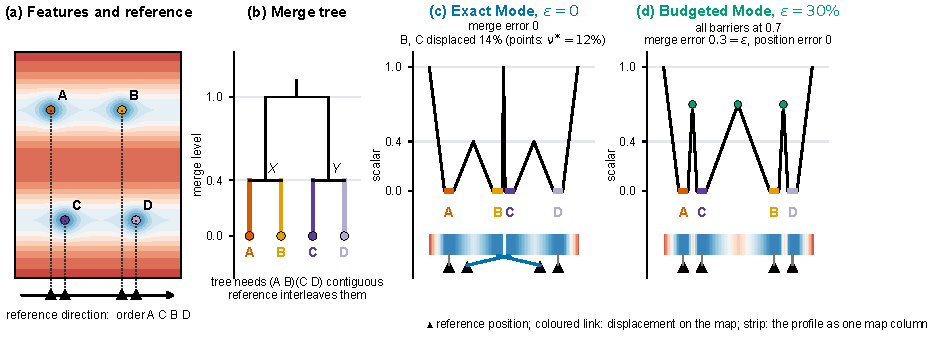
\includegraphics[width=\textwidth]{../figures/fw_concept.pdf}
\caption{Where the positional cost of topology arises, and what releases it. (a) Four minima projected onto one direction appear in the order $A,C,B,D$. (b) The merge tree keeps $(A,B)$ and $(C,D)$ in separate blocks; the conflict sits at their common parent. (c) Keeping the tree exactly forces a displacement of half the overlap of the two blocks' projected ranges: 12\% for points (Theorem~\ref{thm:order}) and 14\% with widths (Theorem~\ref{thm:width}). (d) A merge error of half the parent gap, $\varepsilon=30\%$, lets the blocks interleave (Theorem~\ref{thm:chain}): every displayed merge changes by exactly $\varepsilon$ and no feature moves. Strips: each profile as one column of the temporal map. \todo{relabel ``Exact Mode''/``Budgeted Mode'' as ``exact topology''/``merge error $\varepsilon$''; highlight the conflicting node in (b)}}
\label{fig:concept}
\end{figure*}
\subsection{Merge Trees and Their Profiles}
For a sampled field $f_t:D\to\mathbb{R}$ on a 2D or 3D domain, the merge tree $T_t$ records how sublevel sets join as the threshold rises: minima create components and saddles join them~\cite{Tierny:2018:TTK}. Negating the field gives maxima. A leaf $i$ is an extremum at location $p_i^t$; its support $S_i^t$ is the extremum and the regular samples of its leaf arc. Write $\mathcal{D}(v)$ for the leaves below node $v$ and $h(v)$ for its level. The merge matrix $V_{ij}^t=h(\lca(i,j))$, $V_{ii}^t=f_t(p_i^t)$, determines the tree.

A one-dimensional profile places the extrema at anchors in some leaf order and fills the intervals and gaps with samples of the leaf arcs and the paths to their lowest common ancestors~\cite{Koepp:2023:TMTM,STMTM:2026}. The largest profile value between two anchors is their displayed merge level, so the profile shows the tree exactly only if every subtree occupies one contiguous block. Stacking the profiles along time gives the temporal map.

\subsection{Maps as Hierarchy-Constrained Interval Layouts}
A map frame is $M_t=(\pi_t,x_t,\psi_t)$: a leaf order, anchors and a profile on a canvas $[0,L]$. Each feature occupies an interval of width $W_i$ that contains its anchor; intervals are disjoint with gap $g$, and an anchor may sit at most $\rho W_i/2$ from its interval centre. A \emph{spatial reference} is one unit direction $a$ and origin $o$, fixed for the whole sequence, and the reference of a feature is its projected location
\begin{equation}\label{eq:reference}
 q_i^t=\langle a,p_i^t\rangle-o\in[0,L].
\end{equation}
The direction may be a physical axis or estimated from feature motion (Section~\ref{sec:attain}).

\subsection{Two Fidelities}
\emph{Topology.} The merge error of a profile is the largest change of a displayed merge level, $\dtop(\psi_t,T_t)=\max_{i,j}|V^{\psi_t}_{ij}-V^t_{ij}|$, with $V^\psi_{ij}$ the largest profile value between the anchors of $i$ and $j$. For fixed leaf labels that cover every leaf it equals the labelled interleaving distance, which bounds the bottleneck distance of the persistence diagrams~\cite{Munch:2019:LINF,Gasparovic:2024:IID,Morozov:2013:IDMT}. We report it as NMLE, $\dtop/\Delta_F$ for the scalar range $\Delta_F$, and write $\eta=\varepsilon\Delta_F$ for an allowance $\varepsilon$.

\emph{Position.} The worst displacement of a frame is $\|x-q\|_\infty$. For a fixed order $\pi$, the smallest worst displacement over all interval layouts is
\begin{equation}\label{eq:tau}
 \tau(\pi)=\min_{(x,z)\in\mathcal{L}(\pi)}\|x-q\|_\infty,
\end{equation}
a minimax linear program over the layout set $\mathcal{L}(\pi)$. To compare maps with different widths and scales, the order error
\begin{equation}\label{eq:nroe}
 \nroe(\pi)=\frac{1}{2L}\max_{j\le k}\,[q_{\pi(j)}-q_{\pi(k)}]^+
\end{equation}
is the smallest worst displacement of points placed in order $\pi$, divided by $L$; it depends on the order alone.

\subsection{Existing Maps in the Model}
\begin{table}[t]
\caption{Existing linearizations in the common model. Every method fixes a leaf order and positions; only some keep the merge tree, and none of the merge tree maps fixes the direction of its axis.}\label{tab:methods}
\centering\scriptsize\setlength{\tabcolsep}{2.5pt}
\begin{tabular}{@{}p{0.17\columnwidth}p{0.33\columnwidth}p{0.25\columnwidth}p{0.17\columnwidth}@{}}\toprule
Method & Leaf order & Axis position & Merge error\\\midrule
TMTM~\cite{Koepp:2023:TMTM} & traversal, temporal overlap & sample traversal & 0\\
ST-MTM~\cite{STMTM:2026} & tree-constrained OLO, concordance & relative distances & 0\\
OLO~\cite{BarJoseph:2001:OLO} & adjacent centroid distance & order only & 0\\
Hilbert, Morton & curve rank of extrema & curve rank & 8--40\%\\
Projection & reference order & $x=q$ & up to 59\%\\
Hovm\"oller & none (averaged) & $q$ & merged\\
Anchored (Sec.~\ref{sec:attain}) & least $\tau$ within $\varepsilon$ & near $q$, capped & $\le\varepsilon$\\\bottomrule
\end{tabular}
\end{table}
Table~\ref{tab:methods} places existing linearizations in this model. TMTM, ST-MTM and optimal leaf ordering keep the tree and choose the order for temporal overlap or spatial proximity; space-filling curves and the projection follow space and break the tree; the Hovm\"oller diagram keeps the coordinate but not the features. Merge tree maps fix no direction, and a mirrored map is an equally valid output, so we evaluate each in the orientation that agrees better with the reference. Every map is thus a point in the plane of merge error and displacement. The question of this paper is the lower boundary of the reachable region: for a given tree, reference and widths, how small can the displacement be at each merge error?

\section{The Positional Cost of Topology}\label{sec:bounds}
We bound the displacement in three steps: for exact topology and points, for finite widths, and for a bounded merge error. All three depend only on the tree, the references and the widths; full proofs are in the Supplementary Material. Within a frame we drop $t$, write $[v]^+=\max(v,0)$ and $[m_X,M_X]$ for the reference range of the leaves of a subtree $X$, and take empty maxima as zero.

\subsection{Exact Topology: Where the Cost Arises}
Exact topology lets the order choose only, at every node, the sequence of its children's blocks. Two sibling blocks $X,Y$ can appear as $X$ before $Y$ or $Y$ before $X$; if their reference ranges overlap, either choice inverts some pairs.
\begin{theorem}[Exact-topology bound]\label{thm:order}
On the tree with equal-level merges joined into one node, every zero-error profile has $\nroe(\pi)\ge\nu^*(T,q)$, where
\begin{equation}\label{eq:nu}
 \nu^*(T,q)=\frac{1}{2L}\max_v\max_{\substack{X,Y\in\mathrm{ch}(v)\\X\ne Y}}
 [\min(M_X-m_Y,M_Y-m_X)]^+.
\end{equation}
Ordering the children of every node by the midpoints of their reference ranges attains $\nu^*$ in $O(n\log n)$ time.
\end{theorem}
The maximizing node $v$ and pair $X,Y$ say \emph{where} the cost arises: at the merge of two subtrees whose projected ranges overlap. The value says \emph{how much}: half the overlap that remains in the cheaper of the two orientations. Because midpoint ordering attains $\nu^*$ on the same tree, any order error above $\nu^*$ is chosen by an order rule rather than forced by the tree.

\subsection{Finite Widths}
Features occupy intervals, so blocks must also be packed. For a leaf set $S$ let $H_i=\rho W_i/2$, $\ell_i=q_i-W_i/2-H_i$, $h_i=q_i+W_i/2+H_i$ and $s_i=W_i+g$, and define
\begin{equation}\label{eq:packing}
\begin{aligned}
 A(S)&=\max_{a\in S}\Bigl(\ell_a+\textstyle\sum_{i\in S,\,\ell_i\ge\ell_a}s_i\Bigr),\\
 B(S)&=\max_{b\in S}\Bigl(\textstyle\sum_{i\in S,\,h_i\le h_b}s_i-h_b\Bigr).
\end{aligned}
\end{equation}
For disjoint leaf sets let $\omega(X,Y)=\tfrac12\min\{A(X)+B(Y),A(Y)+B(X)\}-\tfrac g2$, the cheaper orientation of two packed blocks, and let $E_\partial=\max\{0,B(\mathcal{F})-g,A(\mathcal{F})-g-L\}$ account for the canvas ends.
\begin{theorem}[Width-aware bound]\label{thm:width}
For every exact-topology interval layout,
\begin{equation}\label{eq:widthbound}
 \|x-q\|_\infty\ge\tau(\pi)\ge\mathcal{B}_w=\max\{E_\partial,\max_{(X,Y)}\omega(X,Y)\},
\end{equation}
the maximum running over pairs of sibling blocks. With zero widths and gaps, $\mathcal{B}_w=L\nu^*$.
\end{theorem}
The width bound need not be attained; $\tau(\pi)$ is the attained minimum for a given order.

\subsection{A Bounded Merge Error: What Releases the Cost}
A merge error lets blocks interleave, but only up to a point. If leaf $k$ lies between two leaves of node $u$, the displayed merges satisfy $V^\psi_{ik}\le V^\psi_{ij}$, so with $\dtop\le\eta$ the true merge of $k$ with $u$ is at most $h(u)+2\eta$. Let $A_\eta(u)$ be the highest ancestor of $u$ with $h(A_\eta(u))-h(u)\le2\eta$: only leaves below $A_\eta(u)$ may enter the block of $u$. Let $\mathcal{P}_\eta$ contain the pairs $(\mathcal{D}(u),\{k\})$ with $k\notin\mathcal{D}(A_\eta(u))$ and the pairs $(\mathcal{D}(u),\mathcal{D}(w))$ of internal nodes with $\mathcal{D}(w)\cap\mathcal{D}(A_\eta(u))=\varnothing$ and $\mathcal{D}(u)\cap\mathcal{D}(A_\eta(w))=\varnothing$, and let $\kappa(X,Y)=[\min(M_X-m_Y,M_Y-m_X)]^+/(2L)$.
\begin{theorem}[Bounded-topology bound]\label{thm:chain}
Every profile with $\dtop\le\eta$ keeps each pair in $\mathcal{P}_\eta$ in one orientation. Hence $\nroe(\pi)\ge C_\eta=\max_{\mathcal{P}_\eta}\kappa$ and, for interval layouts, $\tau(\pi)\ge C_{w,\eta}=\max\{E_\partial,\max_{\mathcal{P}_\eta}\omega\}$.
\end{theorem}
The theorem says \emph{what releases} a conflict: a subtree may interleave with its sibling once twice the allowance reaches the gap between its own merge level and its parent's. Conflicts at deep merges therefore stay expensive, while conflicts between subtrees that merge just below their parent are released by a small allowance. Flattening every parent gap of at most $2\eta$ gives a second valid bound; neither dominates, and we report the larger.

\subsection{A Ledger of Positional Error}
For any interval layout that keeps the tree, the bounds split its worst displacement into nonnegative parts,
\begin{equation}\label{eq:ledger}
\begin{split}
\|x-q\|_\infty={}&\underbrace{L\nu^*}_{\text{hierarchy}}+\underbrace{(\mathcal{B}_w-L\nu^*)}_{\text{widths}}\\
&+\underbrace{(\tau(\pi)-\mathcal{B}_w)}_{\text{order}}+\underbrace{(\|x-q\|_\infty-\tau(\pi))}_{\text{placement}},
\end{split}
\end{equation}
and its order error into $\nu^*$ and the excess $\nroe(\pi)-\nu^*$. With an allowance, $C_\eta$ and $C_{w,\eta}$ replace $\nu^*$ and $\mathcal{B}_w$. The first two parts are properties of the data, the widths and the direction; the last two are choices of the method. The bounds need no layout: in Python they take at most 5.5\,ms per frame, so they can be evaluated for a candidate direction before any map is drawn.

\section{Attaining the Bounds}\label{sec:attain}
\begin{figure}[t]
\centering
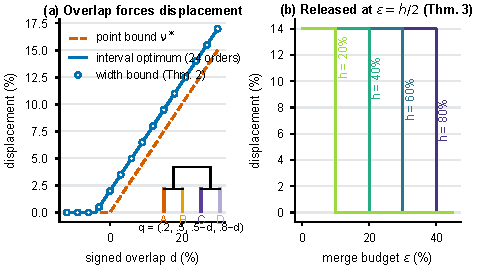
\includegraphics[width=\columnwidth]{../figures/anchor_controlled_bounds.pdf}
\caption{The bounds are exact on controlled trees. Two sibling pairs with references $(0.2,0.5,0.5-d,0.8-d)$. (a) As the overlap $d$ grows, the width bound (circles) equals the optimum over all 24 leaf orders. (b) At $d=24\%$, the 14\% displacement disappears exactly when the allowance reaches half the parent gap $h$, for all four gaps.}
\label{fig:controlled}
\end{figure}
To test whether the bounds can be reached, and to obtain maps whose positional error is known, we use a construction that follows them, which we call AnchorMTM; details are in the Supplementary Material.

\emph{Reference.} By default the direction maximizes the squared projected motion of matched extrema: the leading eigenvector of $\sum\Delta p_i^t(\Delta p_i^t)^\top$ over consecutive-frame matches of leaf supports~\cite{STMTM:2026}. An analyst may supply a physical direction instead.

\emph{Order within a budget.} Each frame starts from the exact tree and its midpoint order, which attains $\nu^*$. Further candidates flatten every parent gap below $2\eta$ or release only the sibling pair that realizes the current bound; a width-aware local search refines the best structures, always including the exact tree. Every candidate is checked against the \emph{original} merge matrix: for a fixed order the least merge error $\delta^*(\pi)$ has a closed form, attained by optimal barriers (Supplementary Material), and candidates with $\delta^*(\pi)>\eta$ are rejected. Among the rest, the order with the least $\tau$, then the least NROE, is selected. A relaxation is thus used only where it lowers the displacement, and the exact tree remains a candidate in every frame.

\emph{Placement and verification.} For the selected order, a convex quadratic program places anchors and intervals near the references and the projected motion, with the worst displacement capped at $\tau(\pi)+\beta_0$. The profile is filled as in prior maps~\cite{Koepp:2023:TMTM,STMTM:2026}, barriers are set to the optimal values, and the rendered merge error is checked against $\varepsilon$.

\section{Characterizing the Cost}\label{sec:experiments}
\subsection{Setup}
\paragraph{Data.} The main benchmark has seven sequences and 917 frames: ERA5 sea-level pressure (Storms, 118 frames)~\cite{Hersbach:2020:ERA5}, wildfire radiative power (30)~\cite{Franke:2021:1DP}, outgoing longwave radiation (OLR, 60)~\cite{NOAA:OLR}, PM$_{2.5}$ (366)~\cite{Dong:2026:PM25}, the synthetic Ring of TMTM (40)~\cite{Koepp:2023:TMTM}, and the Tangaroa (201) and Cylinder (102) flows~\cite{Popinet:2004:Tangaroa,Camarri:2005:Cylinder,Weinkauf:SquareCylinder}. All maps share fields, trees, supports, correspondences and references. For a comparison on the inputs of ST-MTM itself, we also use its four planar inputs, Gaussian, Ring, Wildfires and Storms (64, 40, 32 and 744 frames), reconstructed locally because the authors' processed arrays are unavailable.

\paragraph{Methods.} TMTM uses our port of its official implementation, which matches the official core in all 3127 arc intervals of the planar sequences. ST-MTM has no public code; our implementation follows its Sections 4.1--4.2, meets the optimality conditions of its programs (relative KKT residuals below $10^{-6}$), and uses one setting on all sequences; we also sweep its reordering threshold. Optimal leaf ordering~\cite{BarJoseph:2001:OLO}, Hilbert and Morton curves, the projection and, for OLR, a Hovm\"oller diagram complete the comparison. To compare objectives under equal widths, the Supplementary Material also solves two objectives modelled on TMTM and ST-MTM in our interval model; they do not reproduce the original methods.

\paragraph{Measures.} Merge error is NMLE (Section~\ref{sec:model}); position is NROE, the worst ($E_\infty$) and pooled mean ($E_{\mathrm{pool}}$) of $|x_i-q_i|/L$, and NPE, the worst per-frame value averaged over frames. To credit ST-MTM's objective we also report its scale-normalized stress (SNS) and trustworthiness (TW)~\cite{Smelser:2025:Scale,Venna:2001:NP}.

\subsection{The Bounds Are Tight}
On controlled trees, each bound isolates one cause (Fig.~\ref{fig:controlled}). We fix two sibling pairs merging at $0.4$ below a root at $1$ and vary the signed overlap $d$ of their reference ranges from $-0.12$ to $0.30$; across 43 overlaps and four widths, we compare the bounds with all 24 leaf orders, each placed by an independent minimax program. The tree alone forces $\nu^*=\max(0,d)/2$; with widths $0.06$, gap $0.01$ and $\rho=0.5$, the width bound, the construction and the exhaustive optimum coincide at $\tau=\max(0,(d+0.04)/2)$. An allowance removes the conflict exactly at $2\varepsilon=h$ for all four parent gaps tested.

On real trees, the selected exact-topology order attains the width bound on 606 of the 614 planar frames, so on these frames no exact-topology map has a smaller worst displacement; at $\varepsilon=10\%$ the count is 596, and under halved or doubled widths and gaps it stays within 578--608. Volumetric trees are harder: 81 of 102 Cylinder and 27 of 201 Tangaroa frames, where the remaining gap may lie in the bound or in the search. On Tangaroa at $\varepsilon=5\%$, the bounded-topology bound with widths certifies 7.40\% against an attained 8.10\%, where flattening certifies only 0.38\%.

\subsection{How Much of the Error of Existing Maps Is Forced}
\begin{figure*}[t]
\centering
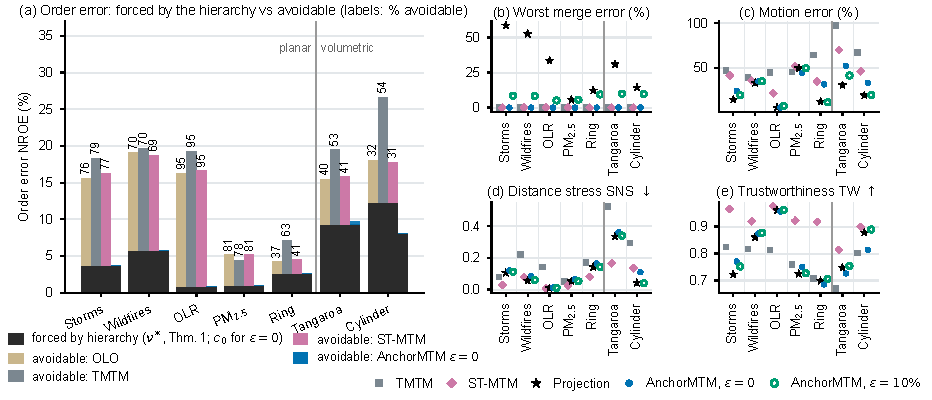
\includegraphics[width=\textwidth]{../figures/fw_compare.pdf}
\caption{Most of the order error of topology-preserving maps is not forced by the tree. (a) Order error of optimal leaf ordering, TMTM and ST-MTM, each in its better mirror, split into the part forced by the hierarchy ($\nu^*$, black) and the excess chosen by each order rule; labels give the excess in percent. (b) Worst merge error: maps that follow space break the tree. (c) Motion error. (d, e) ST-MTM's distance measures, which it optimizes. \todo{keep (a) and (b) in the paper and move (c)--(e) to the Supplementary Material if space is needed}}
\label{fig:ledger}
\end{figure*}
Theorem~\ref{thm:order} splits the order error of every topology-preserving map into the forced $\nu^*$ and an excess that the midpoint order of the same tree removes (Fig.~\ref{fig:ledger}a). On the four real planar sequences the forced part is 0.9--5.8\% of the axis, and the excess is 69--95\% of the order error of optimal leaf ordering, TMTM and ST-MTM alike. On Ring and the two volumes (forced part 2.7--12.2\%), the excess is 53--63\% for TMTM and 31--41\% for the two distance-based orders. The excess is common to these order rules rather than specific to one method, and it is robust to ST-MTM's only order parameter: over its reordering threshold the share stays within 53--95\%, and within 37--61\% on Ring. Space-filling curves show the opposite trade: their extrema orders reach an order error of 0.3--12.6\%, sometimes below $\nu^*$, but only by changing merge levels by 8--40\% of the scalar range, and the projection by up to 59\% (Fig.~\ref{fig:ledger}b).

\subsection{Where the Cost Arises and What Relaxing Buys}
\begin{figure*}[t]
\centering
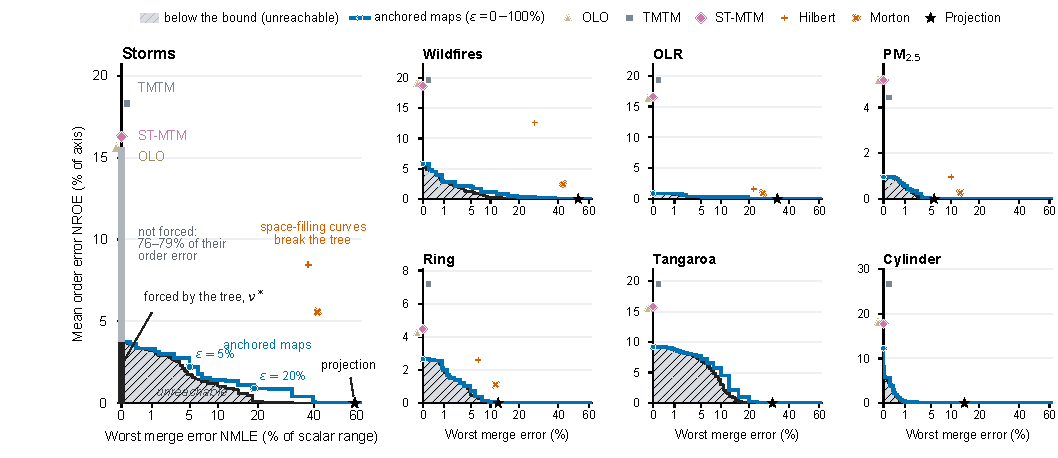
\includegraphics[width=\textwidth]{../figures/fw_plane.pdf}
\caption{The position--topology plane: no map can enter the grey region, topology-preserving maps lie far above it, and maps that follow the bounds run along its edge. Every map of a sequence is one point: its worst merge error over all frames (horizontal, square-root scale) and its mean order error (vertical). Grey: below the frame-averaged bound of Theorems~\ref{thm:order} and~\ref{thm:chain}; no map with that worst merge error has a smaller mean order error. Blue: the construction of Section~\ref{sec:attain} at allowances $\varepsilon$ from 0 to 100\%. TMTM, ST-MTM and optimal leaf ordering keep the tree and lie at zero merge error (offset slightly for legibility), each in its better mirror; Hilbert and Morton curves (planar sequences only) and the projection follow space and break the tree. On Storms, OLR, PM$_{2.5}$ and Ring, enumerating all leaf orders shows that the blue line is the exact optimum, so the band between it and the grey region lies in the bound.}
\label{fig:plane}
\end{figure*}
Figure~\ref{fig:plane} places every map of each sequence in the position--topology plane. Maps that keep the tree sit on the vertical axis, far above the grey region; maps that follow space reach low order error only far to the right. The construction runs along the edge of the grey region: at zero merge error it attains $\nu^*$ on every sequence, and on the four sequences whose frames have at most eight leaves it equals the exhaustive optimum at every tested allowance on all frames but one. Where it stays above the grey region there, the bound, not the construction, is loose.

Theorem~\ref{thm:chain} predicts the shape of the edge: a conflict is released once twice the allowance reaches the gap above the conflicting subtree, so the depth of the conflicting merges decides how fast position can be bought back. Where they merge just below their parent, small allowances suffice: on Cylinder, merge changes below $10^{-6}$ of the scalar range, at the precision of the stored data, already lower the forced order error from 12.24\% to 6.15\%, and 1\% lowers it to 0.23\%; on Wildfires, 1\% halves it, from 5.80\% to 2.77\%. Where they merge deep, position is expensive: on Tangaroa it stays above 7\% up to $\varepsilon=5\%$, and on Storms above 1.4\% up to 10\%. The worst displacement with widths behaves alike (Supplementary Material): on Cylinder 1\% lowers it from 27.00\% to 5.27\%, while on Storms it stays above 18\% up to $\varepsilon=20\%$. The cost is also concentrated in time: on Storms at $\varepsilon=10\%$, the allowance is used in 31 of 118 frames, with a mean merge error of 0.90\% and at most 8.51\%. \todo{optional new analysis: distribution over frames of the parent gap of the bound-realizing pair, i.e., the allowance that releases each frame's conflict}

\subsection{The Direction Changes the Cost}
\begin{figure}[t]
\centering
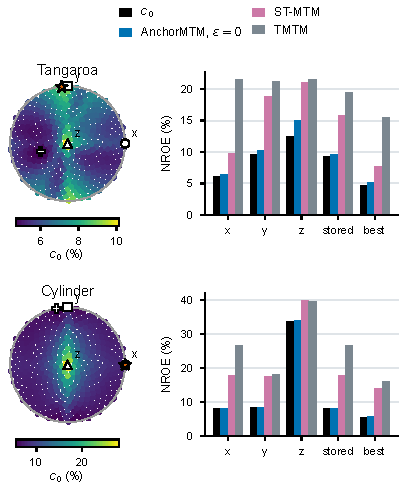
\includegraphics[width=\columnwidth]{../figures/fw_direction.pdf}
\caption{The forced cost depends on the direction and can be read before a map is drawn. Left: mean exact-topology bound over 400 directions of the hemisphere (equal-area projection; centre $z$, rim the $xy$ plane); markers: coordinate axes, the stored direction (star) and the smallest bound (cross). Right: the bound and the mean order error of the construction at $\varepsilon=0$, ST-MTM and TMTM in key directions.}
\label{fig:direction}
\end{figure}
In 3D the forced cost depends strongly on the direction (Fig.~\ref{fig:direction}). Over 400 sampled directions, the mean bound ranges from 4.70\% to 10.14\% on Tangaroa and from 5.49\% to 28.15\% on Cylinder. The direction of dominant motion is not necessarily cheap: on Tangaroa only 4 of the 400 directions have a higher bound, and the $x$ axis would lower it from 9.24\% to 6.09\%. In every key direction the construction stays within 0.6 percentage points of the bound (2.6 on the Tangaroa $z$ axis), while TMTM and ST-MTM stay far above it.

\subsection{Reading Maps with a Known Error}
\begin{table*}[t]
\centering
\caption{Five-dataset comparison. Bold/underline mark best/second distinct values per dataset; ties share emphasis. Curves use fixed default orientations.}
\label{tab:quantitative-final}
\footnotesize
\setlength{\tabcolsep}{1.5pt}
\renewcommand{\arraystretch}{0.85}
\begin{tabular*}{\textwidth}{@{\extracolsep{\fill}}l*{12}{c}lccc@{}}
\toprule
\multirow{2}{*}{Dataset} & \multicolumn{3}{c}{Hilbert} & \multicolumn{3}{c}{Morton} & \multicolumn{3}{c}{TMTM} & \multicolumn{3}{c}{ST-MTM} & \multicolumn{4}{c}{AnchorMTM (ours)} \\
\cmidrule(lr){2-4}\cmidrule(lr){5-7}\cmidrule(lr){8-10}\cmidrule(lr){11-13}\cmidrule(lr){14-17}
 & SNS$\downarrow$ & TW$\uparrow$ & NPE$\downarrow$ & SNS$\downarrow$ & TW$\uparrow$ & NPE$\downarrow$ & SNS$\downarrow$ & TW$\uparrow$ & NPE$\downarrow$ & SNS$\downarrow$ & TW$\uparrow$ & NPE$\downarrow$ & Mode & SNS$\downarrow$ & TW$\uparrow$ & NPE$\downarrow$ \\
\midrule
\multirow{2}{*}{Gaussian} & \multirow{2}{*}{$0.1117$} & \multirow{2}{*}{$0.6719$} & \multirow{2}{*}{$0.7557$} & \multirow{2}{*}{$\underline{0.0393}$} & \multirow{2}{*}{$0.8333$} & \multirow{2}{*}{$0.7359$} & \multirow{2}{*}{$0.2500$} & \multirow{2}{*}{$0.7700$} & \multirow{2}{*}{$\underline{0.1118}$} & \multirow{2}{*}{$0.0600$} & \multirow{2}{*}{$\mathbf{1.0000}$} & \multirow{2}{*}{$0.1154$} & Exact & $\mathbf{0.0353}$ & $\underline{0.9323}$ & $\mathbf{0.0089}$ \\
 &  &  &  &  &  &  &  &  &  &  &  &  & Balanced & $\mathbf{0.0353}$ & $\underline{0.9323}$ & $\mathbf{0.0089}$ \\
\multirow{2}{*}{Ring} & \multirow{2}{*}{$\mathbf{0.1252}$} & \multirow{2}{*}{$\mathbf{0.9048}$} & \multirow{2}{*}{$0.5941$} & \multirow{2}{*}{$0.1489$} & \multirow{2}{*}{$0.7619$} & \multirow{2}{*}{$0.6033$} & \multirow{2}{*}{$0.2800$} & \multirow{2}{*}{$0.6800$} & \multirow{2}{*}{$0.1756$} & \multirow{2}{*}{$0.2100$} & \multirow{2}{*}{$\underline{0.8800}$} & \multirow{2}{*}{$0.2463$} & Exact & $0.1485$ & $0.8571$ & $\underline{0.0471}$ \\
 &  &  &  &  &  &  &  &  &  &  &  &  & Balanced & $\underline{0.1334}$ & $0.8571$ & $\mathbf{0.0395}$ \\
\multirow{2}{*}{Wildfires} & \multirow{2}{*}{$0.1883$} & \multirow{2}{*}{$0.8303$} & \multirow{2}{*}{$0.3641$} & \multirow{2}{*}{$0.1304$} & \multirow{2}{*}{$0.8758$} & \multirow{2}{*}{$0.1560$} & \multirow{2}{*}{$0.4400$} & \multirow{2}{*}{$0.8800$} & \multirow{2}{*}{$0.2280$} & \multirow{2}{*}{$0.2400$} & \multirow{2}{*}{$\underline{0.9100}$} & \multirow{2}{*}{$0.3180$} & Exact & $\mathbf{0.0426}$ & $\mathbf{0.9136}$ & $\underline{0.0131}$ \\
 &  &  &  &  &  &  &  &  &  &  &  &  & Balanced & $\underline{0.0447}$ & $0.8989$ & $\mathbf{0.0116}$ \\
\multirow{2}{*}{Storms} & \multirow{2}{*}{$0.1290$} & \multirow{2}{*}{$0.7403$} & \multirow{2}{*}{$0.3705$} & \multirow{2}{*}{$0.1180$} & \multirow{2}{*}{$0.7251$} & \multirow{2}{*}{$0.3468$} & \multirow{2}{*}{$0.3400$} & \multirow{2}{*}{$0.7100$} & \multirow{2}{*}{$0.5753$} & \multirow{2}{*}{$0.2100$} & \multirow{2}{*}{$\mathbf{0.9400}$} & \multirow{2}{*}{$0.4579$} & Exact & $\underline{0.0790}$ & $0.8463$ & $\underline{0.0399}$ \\
 &  &  &  &  &  &  &  &  &  &  &  &  & Balanced & $\mathbf{0.0743}$ & $\underline{0.8766}$ & $\mathbf{0.0140}$ \\
\multirow{2}{*}{PM2.5} & \multirow{2}{*}{$0.2386$} & \multirow{2}{*}{$\mathbf{0.8887}$} & \multirow{2}{*}{$0.8090$} & \multirow{2}{*}{$\underline{0.1760}$} & \multirow{2}{*}{$\underline{0.8277}$} & \multirow{2}{*}{$0.8823$} & \multirow{2}{*}{$0.3018$} & \multirow{2}{*}{$0.7781$} & \multirow{2}{*}{$0.5241$} & \multirow{2}{*}{$0.1897$} & \multirow{2}{*}{$0.8224$} & \multirow{2}{*}{$0.5577$} & Exact & $0.1964$ & $0.7884$ & $\underline{0.1390}$ \\
 &  &  &  &  &  &  &  &  &  &  &  &  & Balanced & $\mathbf{0.1636}$ & $0.7657$ & $\mathbf{0.0468}$ \\
\bottomrule
\end{tabular*}
\vspace{2pt}
\begin{minipage}{\textwidth}\footnotesize For the original four inputs, TMTM/ST-MTM Temporal SNS/TW are published values; other entries are local measurements. Author inputs and coverage are unconfirmed. Local TW coverage (Gaussian/Ring/Wildfires/Storms) is 64/64, 1/40, 4/32, 11/744; ineligible frames are omitted. Published TW has two-decimal precision. Mode applies only to AnchorMTM. PM2.5 uses 744 shared-input local frames (TW $k=1$, full coverage); its Balanced mode uses the fixed exploratory 5\% case budget, without validation-set budget selection. ST-MTM uses the Storms preset with start frame 0; PM2.5 baseline metrics are all recomputed.\end{minipage}
\end{table*}

A map that attains the bound shows features where they are up to a known error. On OLR (Fig.~\ref{fig:teaser}), the Hovm\"oller diagram resolves a separate dip within 2\% of the reference for only 59\% of the 264 minima, 32\,W\,m$^{-2}$ too shallow on average, because minima at similar positions but different latitudes merge; the exact-topology anchored map shows 94\% of them, 93\% at their exact values, with their nesting. Motion follows: the anchored maps show fewer approach and separation events in the wrong direction than TMTM and ST-MTM on every sequence, by wide margins on Storms (24\% against 41--47\%) and OLR (5.4\% against 21--45\%).

On the inputs of ST-MTM (Table~\ref{tab:quantitative-final}), anchored maps have 73--96\% lower NPE than same-input TMTM and ST-MTM at zero merge error, and 77--98\% lower with an allowance chosen on the first quarter of each sequence; every map stays within its allowance. Position and relative distance are different readings: ST-MTM's published trustworthiness is higher on Gaussian, Ring and Storms and comparable on Wildfires (published to two decimals, from the authors' inputs), and on the main benchmark it has the best TW on all seven sequences and the best SNS on five. \todo{decide whether the Storms allowance sweep (current Fig.~6, without the ``Improvement'' arrows) or the Tangaroa position plot enters the paper}

\section{Discussion and Limitations}\label{sec:discussion}
\paragraph{What the bounds are for.} The bounds turn ``some distortion is unavoidable'' into a number per frame. They tell an analyst how far a displayed feature may be from its location, they tell a method designer how much of a map's error is the method's own, and they let a direction be compared with another before any map is drawn. Order error above $\nu^*$ is always removable without changing the tree; the width-aware and bounded-topology bounds need not be attained, so an excess above them may lie in the bound.

\paragraph{Position is one spatial reading.} Relative distances, which ST-MTM preserves, and neighborhoods answer different questions; a fixed direction preserves neither, and one-dimensional distance preservation has its own unavoidable error~\cite{STMTM:2026}, which our bounds do not quantify. One direction also encodes one coordinate only; reading a 2D position needs a second, time-aligned map along another direction, each with its own bound.

\paragraph{Limitations.} The forced cost is defined for the supplied, possibly simplified tree and for one reference; the default direction is estimated offline from tracked extrema and inherits errors of the correspondence. Metric bounds depend on the chosen widths, whereas the order bound does not. The construction's order search is heuristic and attains the bound on fewer volumetric frames. Results on the ST-MTM inputs use local reconstructions of its data, and its published scores cannot be compared on identical inputs. Whether analysts read positions with a stated error more accurately than without one requires a user study~\cite{Kamakshidasan:2021:MM,McNutt:2020:SVM}.

\section{Conclusion}
Temporal merge tree maps must give up some spatial fidelity to keep the merge tree. For position along a fixed direction, we computed how much: the tree and the projected locations alone determine a lower bound, the merges that force it and the merge error that releases it. Existing topology-preserving maps exceed the bound severalfold, and maps that follow it attain it on almost every planar frame. Stating this cost lets a static overview say not only what the features are and how they nest, but also how far each may be from where it is.

\FloatBarrier
\begingroup
\interlinepenalty=10000
\bibliographystyle{abbrv-doi-narrow}
\bibliography{../refs}
\endgroup
\end{document}
